\section{Integrales de línea}

Como se explica en \textcite{openstax_line_integral}, hay dos tipos de integrales de línea: integrales de línea escalares e integrales de línea vectoriales. Las integrales de línea escalares son integrales de una función escalar sobre una curva en un plano o en el espacio. Las integrales de líneas vectoriales son integrales de un campo vectorial sobre una curva en un plano o en el espacio.

\subsection{Integral de línea escalar}

En cálculo de una variable, una integral de Riemann
$$
\int_a^b g(x)\,dx
$$
se construye sumando ``rectángulos'' $g(x_i^\ast)\Delta x$. En el caso de una integral de línea escalar, la idea es la misma, pero en lugar de intervalos en la recta, tenemos trozos de una curva en el espacio.

Sea una curva $C$ parametrizada por:
$$
\mathbf{r}(t) = (x(t), y(t)), \quad a \leq t \leq b.
$$
donde $t$ es el parámetro (como el ``tiempo''). A medida que $t$ cambia de $a$ a $b$, recorremos la curva.

Queremos integrar una función escalar $f(x,y)$ a lo largo de la curva $C$. Primero dividimos la curva en pedacitos pequeños de longitud $\Delta s_i$ (ver figura \ref{fig:curva_c_integral}). En cada pedacito, elegimos un punto cualquiera, llamado $P_i^\ast$. Evaluamos $f(P_i^\ast)$. Multiplicamos por la longitud del pedacito:
$$
f(P_i^\ast)\,\Delta s_i.
$$
La suma de todos esos productos
$$
\sum_{i=1}^n f(P_i^\ast)\Delta s_i
$$
se parece muchísimo a una suma de Riemann.

Cuando los pedacitos se hacen infinitamente pequeños ($\Delta s_i \to 0$), esa suma converge y se define la integral de línea escalar.
\begin{figure}[ht]
  \centering
  \begin{tikzpicture}[
    % Definimos un estilo para los puntos, para no repetir código
    dot/.style={circle, fill=black, inner sep=1.5pt},
    dotast/.style={circle, fill=teal, inner sep=1.5pt}
  ]
    \draw[gray,->] (-1,0) -- (10,0) node[right] {$x$};
    \draw[gray,->] (-0.5,-0.5) -- (-0.5,4) node[above] {$y$};

    \draw[thick, red,
      decoration={
        markings,
        mark=at position 0 with {
          \node (A) [dot, label=right:\footnotesize$a$] {};
        },
        mark=at position 0.03 with {
          \node (PAast) [dotast, label=right:\scriptsize$\color{teal}P_1^\ast$] {};
        },
        mark=at position 0.06 with {
          \node (PA) [dot, label=right:\scriptsize$\color{orange!70!black}P_1$] {};
        },
        mark=at position 0.35 with {
          \node (P1) [dot, label=below:\scriptsize$\color{orange!70!black}P_{i-1}$] {}; 
        },
        mark=at position 0.4 with {
          \node (Pstar1) [dotast, label=below:\scriptsize$\color{teal}P_{i}^*$] {};
        },
        mark=at position 0.45 with {
          \node (P2) [dot, label=below:\scriptsize$\color{orange!70!black}P_i$] {};
        },
        mark=at position 0.5 with {
          \node (Pstar2) [dotast, label=below:\scriptsize$\color{teal}P_{i+1}^*$] {};
        },
        mark=at position 0.55 with {
          \node (P3) [dot, label=below:\scriptsize$\color{orange!70!black}\quad P_{i+1}$] {};
        },
        mark=at position 0.93 with {
          \node (PB) [dot, label=right:\scriptsize$\color{orange!70!black}P_n$] {};
        },
        mark=at position 0.96 with {
          \node (PBast) [dotast, label=right:\scriptsize$\color{teal}P_n^\ast$] {};
        },
        mark=at position 0.999 with {
          \node (B) [dot, label=right:\footnotesize$b$] {};
        }
      },
      postaction={decorate} % Aplica la decoración DESPUÉS de dibujar la curva
    ] 
    (0.5,1) to [out=80,in=90+55] (5,1.5) 
    to [out=-35,in=260] (9,3) node[above left] {C};

    % --- Definir coordenadas primero ---
    \path ($(A)-(0.3,0)$) coordinate (A_up);
    \path ($(PA)-(0.3,0)$) coordinate (PA_up);
    \path ($(P1)+(0,0.3)$) coordinate (P1_up);
    \path ($(P2)+(0,0.3)$) coordinate (P2_up);
    \path ($(P3)+(0,0.3)$) coordinate (P3_up);
    \path ($(PB)-(0.3,0)$) coordinate (PB_up);
    \path ($(B)-(0.3,0)$) coordinate (B_up);

    % --- Dibujar segmentos ---
    \draw[blue, thick] (A_up) -- (PA_up)
      node[midway, left] {\scriptsize$\Delta S_1$};
    \draw[blue, thick] (P1_up) -- (P2_up)
      node[midway, above, xshift=2mm] {\scriptsize$\Delta S_i$};
    \draw[blue, thick] (P2_up) -- (P3_up)
      node[midway, above, xshift=2mm] {\scriptsize$\Delta S_{i+1}$};
    \draw[blue, thick] (B_up) -- (PB_up)
      node[midway, left] {\scriptsize$\Delta S_n$};

    % --- Dibujar líneas conectoras ---
    \draw[blue] (A) -- ($(A_up)-(0.1,0)$);
    \draw[blue] (PA) -- ($(PA_up)-(+0.1,0)$);
    \draw[blue] (P1) -- ($(P1_up)+(0,0.1)$);
    \draw[blue] (P2) -- ($(P2_up)+(0,0.1)$);
    \draw[blue] (P3) -- ($(P3_up)+(0,0.1)$);
    \draw[blue] (PB) -- ($(PB_up)-(0.1,0)$);
    \draw[blue] (B) -- ($(B_up)-(0.1,0)$);
    
  \end{tikzpicture}
  \caption{Curva paramétrica en el plano.}
  \label{fig:curva_c_integral}
\end{figure}


La integral de línea escalar de $f$ a lo largo de la curva $C$ es:
$$
\int_C f(x,y)\, ds.
$$
Aquí $ds$ es el elemento diferencial de longitud de arco. En términos de la parametrización,
$$
ds = \lvert\mathbf{r}'(t)\rvert\,dt = \sqrt{\Big(\frac{dx}{dt}\Big)^2 + \Big(\frac{dy}{dt}\Big)^2}\,dt.
$$
Por lo tanto:
$$
\int_C f(x,y)\, ds \;=\; \int_a^b f(x(t), y(t)) \,\|\mathbf{r}'(t)\|\,dt.
$$

Una integral de línea escalar es la generalización de la integral de Riemann al caso en que el dominio de integración no es un intervalo recto, sino una curva en el espacio. Se construye sumando valores de $f$ en la curva, multiplicados por trozos de longitud de arco, y tomando el límite para cada trozo tendiendo a cero. Para una intuición gráfica se puede consultar el siguiente vídeo: \parencite{scalar_line_integral}.

\subsection{Integral de línea vectorial}

Sea un campo vectorial en el plano
$$
\vec{F}(x,y) = M(x,y)\,\hat{\imath} + N(x,y)\,\hat{\jmath},
$$
y sea $C$ una curva suave (continuamente derivable) parametrizada por un vector de posición
$$
\vec{r}(t) = x(t)\,\hat{\imath} + y(t)\,\hat{\jmath}, \quad \text{con } t \in [a,b].
$$
La integral de línea de $\vec{F}$ a lo largo de $C$ representa, por ejemplo, el trabajo realizado por el campo $\vec{F}$ al mover una partícula a lo largo de la curva $C$. Se define como:
$$
\int_C \vec{F}\cdot d\vec{r}
$$
Para evaluar esta integral, debemos expresar todos los componentes en términos del parámetro $t$.

\begin{enumerate}
    \item \textbf{El campo} $\vec{F}$ se evalúa a lo largo de la curva $C$, por lo que sustituimos $x=x(t)$ y $y=y(t)$:
    $$
    \vec{F}(\vec{r}(t)) = M(x(t),y(t))\,\hat{\imath} + N(x(t),y(t))\,\hat{\jmath}.
    $$

    \item \textbf{El diferencial de trayectoria} $d\vec{r}$ representa un cambio infinitesimal en la posición a lo largo de la curva. Lo obtenemos derivando la parametrización $\vec{r}(t)$ respecto a $t$:
    $$
    d\vec{r} = \frac{d\vec{r}}{dt}\,dt = \vec{r}\,'(t)\,dt = \left( \frac{dx}{dt}\,\hat{\imath} + \frac{dy}{dt}\,\hat{\jmath} \right)\,dt = \big( x'(t)\,\hat{\imath} + y'(t)\,\hat{\jmath} \big)\,dt.
    $$
\end{enumerate}

Ahora, sustituimos ambos en la integral, calculando el producto punto:
\begin{align*}
\int_C \vec{F}\cdot d\vec{r} &= \int_a^b \vec{F}(\vec{r}(t)) \cdot \vec{r}\,'(t)\,dt \\
&= \int_a^b \Big( M(x(t),y(t))\,\hat{\imath} + N(x(t),y(t))\,\hat{\jmath} \Big) \cdot \Big( x'(t)\,\hat{\imath} + y'(t)\,\hat{\jmath} \Big)\,dt
\end{align*}
Resolviendo el producto punto $(\hat{\imath}\cdot\hat{\imath}=1, \hat{\jmath}\cdot\hat{\jmath}=1, \hat{\imath}\cdot\hat{\jmath}=0)$, llegamos a la fórmula computacional:
$$
\int_C \vec{F}\cdot d\vec{r} \;=\; \int_a^b \Big( M(x(t),y(t))\,x'(t) + N(x(t),y(t))\,y'(t) \Big)\,dt.
$$

\textbf{Notación diferencial alternativa:}
Si utilizamos la notación de diferenciales $dx = x'(t)\,dt$ y $dy = y'(t)\,dt$, podemos reescribir la integral paramétrica de forma compacta. 
$$
\int_C \vec{F}\cdot d\vec{r} \;=\; \int_C M(x,y)\,dx + N(x,y)\,dy.
$$
Ambas expresiones son equivalentes, pero la forma paramétrica es la que se utiliza para el cálculo directo.

Si el campo $\vec{F}$ es conservativo, es decir, existe un potencial $\nabla f(x,y)$ tal que
$$
\nabla f(x,y) = \vec{F}(x,y),
$$
entonces:
$$
\int_C \vec{F}\cdot d\vec{r} \;=\; f(\vec{r}(b)) - f(\vec{r}(a)).
$$
Es decir, la integral de línea solo depende de los extremos de la curva, y no de la trayectoria.

\subsubsection{Relación con el Teorema de Green}

Si la curva $C$ es cerrada (recorre el borde de una región $D$ en sentido antihorario), el teorema de Green nos da:
$$
\oint_C \vec{F}\cdot d\vec{r} \;=\; \iint_D \left( \frac{\partial N}{\partial x} - \frac{\partial M}{\partial y} \right)\, dA.
$$
Si $\vec{F}$ es conservativo, entonces se cumple
$$
\frac{\partial N}{\partial x} = \frac{\partial M}{\partial y},
$$
lo que implica que la integral de línea cerrada es cero:
$$
\oint_C \vec{F}\cdot d\vec{r} = 0.
$$
Esto conecta la idea de conservatividad con el teorema de Green. También, puedes obtener mejor intuición visual de la integral de línea vectorial a través del siguiente vídeo: \parencite{vector_line_integral}.

\section{El teorema de Green}

El teorema de Green conecta dos tipos de integrales. Relaciona la integral de línea de un campo vectorial alrededor de una curva cerrada simple $C$ (que es el borde de una región) con una integral doble sobre la región plana $D$ que esa curva encierra.

Supongamos una región $D$ está dividida en muchos cuadrados pequeños (llamados $dA$). Ahora, pensemos en la integral de línea del campo vectorial alrededor de cada uno de esos cuadraditos. La integral de línea la recorremos siempre en sentido antihorario.

Los cuadraditos están pegados unos a otros en el interior de la región. Entonces, todos los cuadraditos internos tienen un lado en común con sus cuadrados vecinos. Al recorrer estos lados comunes, en un momento recorreremos el segmento hacia abajo, y luego, al recorrer el cuadrado del lado, recorreremos el mismo segmento pero hacia arriba, como se muestra en la figura \ref{fig:cuadrados_comunes_greeen}. Esta misma idea sucede con los cuadrados ubicados verticalmente, donde su segmento común es horizontal.

\begin{figure}[ht]
\centering
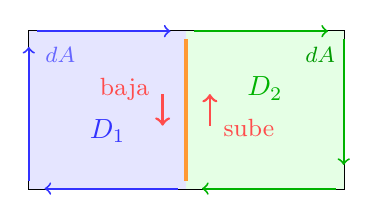
\begin{tikzpicture}
    
    % Región D (forma simple dividida en dos)
    \draw[thick, fill=blue!5] (0,0) rectangle (4,2);
    
    % Línea divisoria (el segmento común)
    \draw[red, line width=2.5pt] (2, 0) -- (2, 2);
    
    % Etiqueta del segmento común
    \node[red, right=3pt, font=\Large] at (2, 1) {I};
    
    % Sombreado diferente para cada mitad
    \fill[blue!10] (0,0) rectangle (2,2);
    \fill[green!10] (2,0) rectangle (4,2);
    
    % Contornos de cada cuadrado con flechas antihorarias
    % Cuadrado izquierdo (azul)
    \draw[->,blue!80, line width=0.7pt] (0.1, 2) -- (1.8, 2);
    \draw[->,blue!80, line width=0.7pt] (1.9, 0) -- (0.2, 0);
    \draw[->,blue!80, line width=0.7pt] (0, 0.1) -- (0, 1.8);
    
    % Cuadrado derecho (verde)
    \draw[->,green!70!black, line width=0.7pt] (2.1, 2) -- (3.8, 2);
    \draw[->,green!70!black, line width=0.7pt] (4, 1.9) -- (4, 0.3);
    \draw[->,green!70!black, line width=0.7pt] (3.9, 0) -- (2.2, 0);
    
    \draw[orange!80, line width=1.3pt] (2, 1.9) -- (2, 0.1);

    % Etiquetas de los cuadrados
    \node[blue!80, below] at (1, 1) {$D_1$};
    \node[green!70!black, above] at (3, 1) {$D_2$};
    
    % Flechas grandes indicando dirección en el segmento I
    \draw[->,red!70, line width=1pt] (1.7, 1.2) -- (1.7, 0.8);
    \node[red!70, above left, font=\small] at (1.65, 1) {baja};
    
    \draw[->,red!70, line width=1pt] (2.3, 0.8) -- (2.3, 1.2);
    \node[red!70, below right, font=\small] at (2.35, 1) {sube};
    
    % Etiquetas dA
    \node[blue!60, font=\footnotesize] at (0.4, 1.7) {$dA$};
    \node[green!60!black, font=\footnotesize] at (3.7, 1.7) {$dA$};
    
\end{tikzpicture}
\caption{Al integrar sobre una región $D$ los segmentos internos se cancelan y solo queda la contribución del perímetro exterior.}
\label{fig:cuadrados_comunes_greeen}
\end{figure}

Como el campo vectorial a lo largo del segmento común es el mismo para las dos integrales, pero recorremos el camino en direcciones opuestas, esas dos integrales de línea (solo en ese lado común) se cancelan, ya que tienen el mismo valor pero el signo opuesto.

Todos los lados internos se anulan por pares, y lo único que sobrevive es la ``cáscara'' exterior: el borde $C$ de la región $D$ completa.

Así que, intuitivamente, hemos llegado a esto: la suma de todos los pequeños ``remolinos'' dentro de la región $D$ es igual a la circulación total en el borde exterior $C$. Esta es la esencia del Teorema de Green.

\subsection{Definición del teorema}

Ahora, pongámosle matemáticas a esa idea. El teorema se escribe así:
$$\oint_C (P\,dx + Q\,dy) = \iint_D \left( \frac{\partial Q}{\partial x} - \frac{\partial P}{\partial y} \right) dA$$
Vamos a diseccionar esto, conectándolo con nuestra intuición. 

El lado izquierdo: $\oint_C (P\,dx + Q\,dy)$ es el término que ya conoces, la integral de línea vectorial (o circulación) del campo $\vec{F} = \langle P, Q \rangle$ a lo largo de la curva cerrada $C$. Esta es la circulación total en el borde exterior que no se canceló.

El lado derecho: $\iint_D \left( \frac{\partial Q}{\partial x} - \frac{\partial P}{\partial y} \right) dA$ es una integral doble sobre la región $D$ (la superficie interior). En nuestra analogía, esta es la suma de todos los pequeños remolinos dentro de la región. Justamente $\text{rot }F=Q_x-P_y$, de modo que es la integral del rotacional en cada pequeño $dA$.

\subsection{Aplicación a campos conservativos}

Si el campo $\vec{F}$ es conservativo, la integral de línea sobre cualquier curva cerrada $C$ es cero. 

El Teorema de Green nos da la igualdad:
$$\oint_C (P\,dx + Q\,dy) = \iint_D \left( \frac{\partial Q}{\partial x} - \frac{\partial P}{\partial y} \right) dA$$
Ahora, conectemos las dos ideas:
\begin{enumerate}
\item Sabemos que el lado izquierdo (la integral de línea) debe ser 0 para cualquier curva cerrada $C$, porque el campo es conservativo.
\item Por lo tanto, el lado derecho (la integral doble) también debe ser 0 para cualquier región $D$.
\end{enumerate}

Aquí vemos que si la integral $\iint_D \left( \frac{\partial Q}{\partial x} - \frac{\partial P}{\partial y} \right) dA$ es cero para toda región D posible (sin importar qué tan pequeña o grande la dibujemos)\dots~ ¿qué nos dice eso sobre la propia expresión que estamos integrando?

¿A qué debe ser igual $\left( \frac{\partial Q}{\partial x} - \frac{\partial P}{\partial y} \right)$ en todos los puntos de la región? El Teorema de Green nos permite construir este puente lógico; si $\vec{F}$ es conservativo, por definición, $\oint_C \vec{F} \cdot d\vec{r} = 0$ para cualquier curva cerrada $C$. La única forma de que una integral doble sea cero para toda región posible (grande, pequeña, etc.) es que la función que estamos integrando (el integrando) sea cero en todos los puntos.
Por lo tanto:
$$\frac{\partial Q}{\partial x} - \frac{\partial P}{\partial y} = 0 \implies \frac{\partial Q}{\partial x} = \frac{\partial P}{\partial y}$$

Esto coincide perfectamente con lo que ya sabíamos: si $\vec{F} = \nabla f$ (es decir, $\vec{F} = \langle f_x, f_y \rangle = \langle P, Q \rangle$), entonces la igualdad de las derivadas cruzadas nos dice que forzosamente $P_y = Q_x$.

\subsection{Condiciones Necesarias y Suficientes}

Hemos establecido una condición necesaria: Si un campo $\vec{F}$ es conservativo, necesariamente debe cumplir que $Q_x = P_y$. Ahora, la pregunta inversa: ¿Es esta una condición suficiente? Es decir, si encuentro un campo donde $Q_x = P_y$, ¿puedo garantizar que es conservativo?

La respuesta es ``casi''. Es suficiente siempre y cuando la región $D$ donde el campo está definido no tenga ``agujeros''. A esto se le llama una región simplemente conexa.
